\documentclass[conference]{IEEEtran}
\IEEEoverridecommandlockouts
\usepackage{cite}
\usepackage{amsmath,amssymb,amsfonts}
\usepackage{algorithm}
\usepackage{algpseudocode}
\usepackage{graphicx}
\usepackage{booktabs}
\usepackage{multirow}
\usepackage{xcolor}
\usepackage{tikz}
\usetikzlibrary{arrows.meta,positioning,fit}
\usepackage[hidelinks]{hyperref}
\usepackage{url}

\newcommand{\TODO}[1]{\textcolor{red}{\textbf{TODO:} #1}}
% figure that compiles even before the file is uploaded
\newcommand{\safegraphic}[2]{\IfFileExists{#2}{\includegraphics[width=#1]{#2}}{\fbox{\parbox{#1}{\centering\TODO{add #2}}}}}

\begin{document}

\title{TrialMatch: Criterion-Level Clinical-Trial Eligibility with Cited Evidence, Explicit KV Caching, Tiled Attention and Speculative Decoding}

\author{\IEEEauthorblockN{Abubakar}
\IEEEauthorblockA{Student ID: 23i-0515}}

\maketitle

\begin{abstract}
Matching patients to clinical trials requires checking a patient record against every inclusion and exclusion criterion and justifying each decision. We fine-tune Qwen2.5-1.5B-Instruct with LoRA on the TrialGPT-Criterion-Annotations dataset to output, for one patient note and one criterion, an eligibility label and the IDs of the supporting note sentences. On a fixed patient-level split (37/8/8 patients, seed 42), fine-tuning raises validation accuracy from 0.068 to 0.743 and macro-F1 from 0.082 to 0.552, removes all malformed outputs, and lifts evidence micro-F1 from 0.091 to 0.535; on the held-out test set the selected model reaches \TODO{test accuracy / macro-F1 / evidence F1}. Around the model we implement, from raw forward passes, a KV-cache decoder that is token-identical to uncached decoding and 1.3--5.9$\times$ faster on a T4 GPU (up to 24.5$\times$ in fp32), a tiled online-softmax attention whose largest intermediate is 1024$\times$ smaller than the full score matrix at $N=4096$, and greedy speculative decoding with a 0.5B draft that reproduces the target's output exactly. A local browser application screens a note against a criteria list, shows verbatim evidence, aggregates a rule-based preliminary outcome and exports a report with provenance.
\end{abstract}

\begin{IEEEkeywords}
clinical trial matching, large language models, LoRA, KV cache, online softmax, speculative decoding
\end{IEEEkeywords}

% =====================================================================
\section{Introduction}
Manual pre-screening of patient records against trial eligibility criteria is slow and a recognised bottleneck in trial recruitment~\cite{jin2024trialgpt}. Each trial lists free-text inclusion and exclusion criteria; a screener must decide, for every criterion, whether the record shows the patient meets it, does not meet it, lacks the information, or whether the criterion does not apply, and should point to the part of the record that supports the decision.

TrialGPT~\cite{jin2024trialgpt} showed that GPT-4 can perform this criterion-level matching with explanations. Proprietary models are, however, impractical for patient data that may not leave an institution. We ask whether a small open model (1.5B parameters) that runs on a laptop can learn the same task from the expert annotations released with TrialGPT, and we build the inference stack ourselves to make its cost transparent.

\textbf{Contributions.} (1) A reproducible patient-level split and a leakage-free prompt that uses only the note, criterion type and criterion text. (2) LoRA fine-tuning with completion-only loss, compared before/after on identical rows, with three competing configurations selected on validation only. (3) Criterion-level evaluation of labels \emph{and} cited evidence, with stated rules for empty evidence sets. (4) Hand-written KV-cache decoding, tiled online-softmax attention and greedy speculative decoding, each verified for exactness and benchmarked. (5) A local browser application with evidence display, export and an inference laboratory.

% =====================================================================
\section{Related Work}
\textbf{LLM-based trial matching.} TrialGPT~\cite{jin2024trialgpt} prompts GPT-4 per criterion to produce a relevance explanation, the relevant sentence IDs and an eligibility label, then aggregates criterion scores to rank trials; its criterion-level accuracy approached that of human experts. Our work keeps the per-criterion formulation and the sentence-ID evidence format but replaces the proprietary model by a fine-tuned 1.5B open model, uses the \emph{expert} labels as supervision, and explicitly avoids training on GPT-4 outputs. Unlike TrialGPT we do not rank trials; the overall outcome is a transparent rule over criterion labels.

\textbf{Transformers and parameter-efficient tuning.} The Transformer~\cite{vaswani2017attention} underlies all models used here. Qwen2.5~\cite{qwen2025} uses grouped-query attention (GQA) with two key/value heads, which keeps the KV cache small. LoRA~\cite{hu2022lora} freezes the pretrained weights and learns low-rank updates $W + BA$; QLoRA~\cite{dettmers2023qlora} adds 4-bit quantisation of the frozen weights. At 1.5B parameters the fp16 model and LoRA states fit comfortably in a 16\,GB T4 (4.3\,GB peak in our runs), so quantisation was unnecessary and we use plain LoRA, which avoids quantisation error in the merged model used for inference.

\textbf{Efficient attention.} Milakov and Gimelshein~\cite{milakov2018online} showed that softmax can be computed in one pass by maintaining a running maximum and normaliser. FlashAttention~\cite{dao2022flashattention} combines this with tiling so that the $N\times N$ score matrix is never materialised, keeping tiles in on-chip SRAM. Our tiled kernel implements the same recurrence in PyTorch; it reproduces the memory behaviour but, lacking kernel fusion, not the speed.

\textbf{Speculative decoding.} Leviathan et al.~\cite{leviathan2023fast} and Chen et al.~\cite{chen2023accelerating} let a small draft model propose several tokens that the target verifies in a single forward pass, with a rejection rule that preserves the target distribution. For greedy decoding the rule reduces to accepting the longest prefix on which the draft agrees with the target's argmax, which is what we implement.

% =====================================================================
\section{Methods}
\subsection{Dataset and split}
TrialGPT-Criterion-Annotations (revision \texttt{1cfcafd}) contains 1{,}015 expert-annotated (patient, criterion) pairs over 53 patients and 103 trials~\cite{jin2024trialgpt}; the patients are the SIGIR cohort of TREC Clinical Decision Support case descriptions~\cite{koopman2016test}. Notes are pre-split into numbered sentences; gold evidence is a list of sentence IDs. Inclusion criteria take one of \{included, not included, not enough information, not applicable\}; exclusion criteria one of \{excluded, not excluded, not enough information, not applicable\}. One row with an empty criterion was removed. Following the assignment protocol, the sorted unique patient IDs were shuffled with \texttt{numpy.random.default\_rng(42)} and split 37/8/8 into train/validation/test (602/206/206 rows; Table~\ref{tab:split}). Tests assert disjoint patients, full coverage, and that re-running the split reproduces the manifest byte for byte. The split is by patient; one trial occurs in both train and validation, none in test. The label distribution is highly skewed: ``not excluded'' is 48\% of all rows and the test set contains no ``excluded'' row.

\begin{table}[t]
\centering
\caption{Patient-level split (rows by gold label).}
\label{tab:split}
\begin{tabular}{lrrr}
\toprule
 & Train & Val & Test \\
\midrule
Patients / trials & 37 / 72 & 8 / 16 & 8 / 16 \\
Rows (incl.\ / excl.) & 215 / 387 & 66 / 140 & 75 / 131 \\
included / not included & 88 / 13 & 35 / 3 & 27 / 7 \\
excluded / not excluded & 8 / 291 & 2 / 101 & 0 / 91 \\
not enough information & 174 & 53 & 66 \\
not applicable & 28 & 12 & 15 \\
Empty gold evidence & 348 & 116 & 145 \\
\bottomrule
\end{tabular}
\end{table}

\subsection{Task formulation and prompt}
Each example is rendered with the Qwen chat template. The system message describes the four labels allowed for the criterion's type; the user message contains the numbered note, the criterion type and the criterion text---nothing else (a test asserts that no GPT-4 explanation, GPT-4 label or other annotation column can reach the prompt). The target is compact JSON, \texttt{\{"label": "\ldots", "evidence": [ids]\}}. Prompts are 251--621 tokens and targets 12--37 tokens, so no note is truncated; the application truncates whole trailing sentences if a user note exceeds its 1{,}536-token budget and reports which sentences were dropped.

\subsection{Model choice}
Table~\ref{tab:models} compares the candidates. Qwen2.5-1.5B-Instruct is the target: it is the largest model whose fp16 weights plus a draft model fit a 16\,GB laptop for interactive use, has a 32k context (far above our 621-token prompts) and an Apache-2.0 licence. Qwen2.5-0.5B-Instruct shares the tokenizer exactly (asserted in code), which speculative decoding requires, and serves both as a second fine-tuning candidate and as the draft. Llama-3.2-3B was rejected: 2$\times$ the memory, a gated licence, and no same-tokenizer draft in the planned budget.

\begin{table}[t]
\centering
\caption{Models considered.}
\label{tab:models}
\setlength{\tabcolsep}{3pt}
\begin{tabular}{lccc}
\toprule
 & Qwen2.5-1.5B & Qwen2.5-0.5B & Llama-3.2-3B \\
\midrule
Role & target & 2nd cand./draft & rejected \\
Parameters & 1.54B & 0.49B & 3.2B \\
Layers / hidden & 28 / 1536 & 24 / 896 & 28 / 3072 \\
Q / KV heads, $d_h$ & 12 / 2, 128 & 14 / 2, 64 & 24 / 8, 128 \\
Vocabulary & 151{,}936 & 151{,}936 & 128{,}256 \\
Context & 32k & 32k & 128k \\
Licence & Apache-2.0 & Apache-2.0 & Llama 3.2 \\
fp16 weights & 3.1\,GB & 1.0\,GB & 6.4\,GB \\
KV cache / token (fp16) & 28\,KB & 12\,KB & 112\,KB \\
\bottomrule
\end{tabular}
\end{table}

\subsection{Fine-tuning}
We train LoRA adapters ($r=16$, $\alpha=32$, dropout 0.05) on all attention and MLP projections (18.5M trainable parameters, 1.2\% of the model) with AdamW, learning rate $2\times10^{-4}$, 5\% warm-up and cosine decay, effective batch 16, 3 epochs, gradient clipping at 1.0. The loss is the causal LM loss on the answer tokens only; prompt tokens are masked with $-100$, and logits are computed only for the answer positions (\texttt{logits\_to\_keep}), which a test verifies gives the same loss as the full computation. The T4 has no native bf16, so training uses fp16 autocast with a gradient scaler. After every epoch we compute validation loss and run greedy generation on the full validation set; the checkpoint with the best validation macro-F1 is kept. Competing choices---LoRA rank 8 vs.\ 16, and the 0.5B vs.\ the 1.5B model---were decided on validation only.

\subsection{System architecture}
Fig.~\ref{fig:arch} shows the pipeline. For each criterion the model returns label and IDs; everything else is derived deterministically. Cited IDs are mapped to the note's sentences and shown verbatim; IDs outside the note are reported as unsupported citations and never displayed as evidence. Because the dataset contains no expert explanations and GPT-4 explanations must not be used, explanations are templates filled with the label and the quoted evidence, so they cannot assert facts absent from the note. Missing evidence is never taken as proof: a criterion without evidence is shown as such and ``not enough information'' is listed as missing information. Invalid labels and unparseable outputs are counted as errors and never silently remapped.

\begin{figure}[t]
\centering
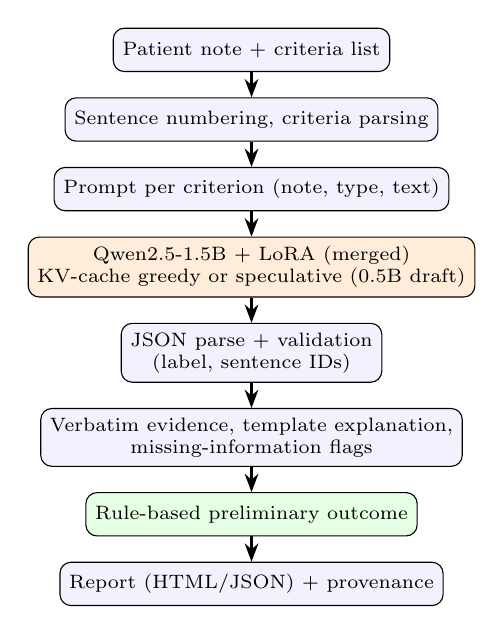
\begin{tikzpicture}[node distance=0.32cm, every node/.style={font=\scriptsize}, box/.style={draw, rounded corners, align=center, minimum width=2.6cm, minimum height=0.55cm, fill=blue!5}, arr/.style={-{Stealth}, thick}]
\node[box] (in) {Patient note + criteria list};
\node[box, below=of in] (seg) {Sentence numbering, criteria parsing};
\node[box, below=of seg] (pr) {Prompt per criterion (note, type, text)};
\node[box, below=of pr, fill=orange!15] (m) {Qwen2.5-1.5B + LoRA (merged)\\KV-cache greedy or speculative (0.5B draft)};
\node[box, below=of m] (js) {JSON parse + validation\\(label, sentence IDs)};
\node[box, below=of js] (ev) {Verbatim evidence, template explanation,\\missing-information flags};
\node[box, below=of ev, fill=green!10] (ag) {Rule-based preliminary outcome};
\node[box, below=of ag] (ex) {Report (HTML/JSON) + provenance};
\foreach \src/\dst in {in/seg,seg/pr,pr/m,m/js,js/ev,ev/ag,ag/ex} \draw[arr] (\src) -- (\dst);
\end{tikzpicture}
\caption{Screening pipeline. Only the orange step uses the neural model.}
\label{fig:arch}
\end{figure}

\textbf{Aggregation.} The overall outcome is a stated rule, presented as preliminary: \emph{Likely ineligible} if any inclusion criterion is ``not included'' or any exclusion criterion is ``excluded''; otherwise \emph{Needs more information} if any criterion is ``not enough information'' or unresolved; otherwise \emph{Potentially eligible}; ``not applicable'' criteria are ignored.

\subsection{Explicit KV-cache decoding}
Both decoders call the model's forward pass directly. The reference re-runs the full sequence at every step without a cache. The cached decoder runs one prefill pass over the prompt into a \texttt{DynamicCache} and then feeds only the newest token. We pass three things explicitly. \emph{Positions:} Qwen2 applies RoPE to keys before they are cached, so cached keys are already rotated with their absolute positions and the new token must receive \texttt{position\_ids} $=$ the number of cached tokens; a wrong position does not crash but silently changes the output. \emph{Mask:} we build the boolean mask ourselves---query $i$ at absolute position $p+i$ may attend key $j$ iff $j\le p+i$; during prefill this is lower-triangular, in a decode step the single query may attend every cached key, so causality is enforced by the cache containing only the past. \emph{Cache growth:} after each step we assert that the cache grew by the number of fed tokens. Per token the cache stores $2\times L\times H_{kv}\times d_h$ values ($2\cdot28\cdot2\cdot128$ = 14{,}336, i.e.\ 28\,KB in fp16), so memory grows linearly while uncached cost grows quadratically in sequence length.

\subsection{Tiled online-softmax attention}
Algorithm~\ref{alg:tiled} processes query tiles of $B_r$ rows against key/value tiles of $B_c$ columns, keeping per query row a running maximum $m$, normaliser $\ell$ and unnormalised output $O$; when a new tile raises the maximum, previous contributions are rescaled by $e^{m_{old}-m_{new}}$. Under causal masking, key tiles lying entirely in the future of a query tile are skipped and only tiles straddling the diagonal are masked (bottom-right aligned, so $N_q\neq N_k$ such as a decode step works). GQA is supported by repeating KV heads. The largest intermediate is one $B_r\times B_c$ score tile instead of $N\times N$.

\begin{algorithm}[t]
\caption{Tiled online-softmax attention (one head)}
\label{alg:tiled}
\begin{algorithmic}[1]
\For{each query tile $Q_i$ ($B_r$ rows)}
\State $m \gets -\infty$, $\ell \gets 0$, $O \gets 0$
\For{each key tile $j$ with keys not all in the future of $Q_i$}
\State $S \gets Q_i K_j^\top / \sqrt{d}$; mask future keys if tile straddles diagonal
\State $m' \gets \max(m, \mathrm{rowmax}(S))$; $P \gets \exp(S - m')$
\State $\alpha \gets \exp(m - m')$
\State $\ell \gets \alpha \ell + \mathrm{rowsum}(P)$; $O \gets \alpha O + P V_j$; $m \gets m'$
\EndFor
\State $O_i \gets O / \ell$
\EndFor
\end{algorithmic}
\end{algorithm}

\subsection{Greedy speculative decoding}
Algorithm~\ref{alg:spec} is built on the cached decoder. Both models are prefilled with the prompt. Each round the draft proposes $k$ tokens greedily; the target scores the last emitted token followed by the $k$ drafts in one forward pass (causal mask over the block, positions continuing from the cache), giving $k+1$ argmaxes $g_0..g_k$. The longest prefix with $d_{i+1}=g_i$ ($n$ tokens) is accepted and $g_n$ is appended---a correction if $n<k$, a free bonus token if $n=k$. Both caches are then cropped to ``all tokens except the last emitted one'' (the target drops $k-n$ entries; the draft drops $k-1-n$, or, if everything was accepted, feeds the never-cached $d_k$ in its next call). Because acceptance compares with the target's own argmax, the output is exactly the target's greedy output; the draft only changes how many target passes are needed.

\begin{algorithm}[t]
\caption{Greedy speculative decoding}
\label{alg:spec}
\begin{algorithmic}[1]
\State prefill target and draft caches with the prompt; $y \gets [\arg\max$ target$]$
\While{$|y| <$ max and last token $\neq$ EOS}
\State $d_{1..k} \gets$ draft greedy continuation from $y$ (cached)
\State $g_{0..k} \gets \arg\max$ target$([y_{-1}, d_1..d_k])$ \Comment{one pass}
\State $n \gets \max\{n : d_{1..n} = g_{0..n-1}\}$
\State $y \gets y + [d_1..d_n, g_n]$
\State crop target cache by $k-n$, draft cache by $k-1-n$
\EndWhile
\end{algorithmic}
\end{algorithm}

\subsection{Application}
The Gradio application runs locally (\texttt{start.command} or \texttt{./run.sh}) and shows a persistent disclaimer. The \emph{Screening} tab accepts free-text or numbered notes and an \texttt{Inclusion:}/\texttt{Exclusion:} criteria list, or loads a held-out test example (with expert labels shown for comparison). Results show a label badge, cited IDs, evidence highlighted in the numbered note, the explanation, missing information, warnings (truncation, unsupported citations) and the aggregated outcome; reports are exported as HTML and JSON with provenance (model, adapter, decoding mode and settings, device, timestamp, input hash, code version). Empty or malformed inputs produce inline messages; unexpected failures are caught so the app keeps running. The \emph{Inference Lab} runs the three decoders and the three attention implementations live and checks token identity and numerical error (Fig.~\ref{fig:app}).

% =====================================================================
\section{Experimental Setup and Metrics}
Training and GPU benchmarks ran on a Google Colab Tesla T4 (16\,GB, compute capability 7.5, CUDA 13.0, PyTorch 2.11, Transformers 5.22.1, PEFT 0.21.2); the application and Mac benchmarks on an Apple M5 laptop (16\,GB, MPS, PyTorch 2.15). All evaluations use greedy decoding (\texttt{do\_sample=False}, repetition penalty 1.0, at most 64 new tokens); Qwen's default sampling configuration is replaced, not merged. Base and fine-tuned models are evaluated on identical rows with identical prompts. The test set was evaluated once, after all choices were frozen on validation.

\textbf{Classification.} Accuracy, per-class precision/recall/F1, macro-F1 and confusion matrices, overall (six labels) and separately for inclusion and exclusion criteria. Macro-F1 averages over labels present in gold or predictions; an invalid or unparseable output counts as wrong.

\textbf{Evidence.} Cited IDs are compared with gold IDs as sets. Micro P/R/F1 pool true/false positives and false negatives over all records; macro values average per record. Empty sets: gold and prediction both empty count as P=R=F1=1; empty gold with non-empty prediction gives P=0, F1=0 and is excluded from the recall mean; non-empty gold with empty prediction gives R=0. Because 56\% of validation rows have empty gold evidence, we also report metrics on non-empty-gold records only.

\textbf{Efficiency.} Device-synchronised wall-clock timing around every timer, warm-up runs, medians over repeats; peak memory from the CUDA allocator (on MPS only sampled after forward passes, a lower bound). Token equality is checked on every configuration; on a mismatch the step and top-1/top-2 logit margin are logged.

% =====================================================================
\section{Results and Discussion}
\subsection{Fine-tuning: before and after}
Table~\ref{tab:val} reports validation results. The base 1.5B model produces well-formed JSON but labels every one of the 140 exclusion rows ``excluded'' (including all 101 ``not excluded'' rows): it reads ``excluded'' as ``the criterion is about an exclusion'' rather than ``the patient meets it'', a polarity confusion that fine-tuning removes completely (the fine-tuned model is correct on all 101). The base 0.5B fails to produce parseable JSON for 136 of 206 rows. Fine-tuning raises accuracy by 0.68 and macro-F1 by 0.47 with no invalid output.

\begin{table}[t]
\centering
\caption{Validation results (206 rows; selection by macro-F1).}
\label{tab:val}
\setlength{\tabcolsep}{2.5pt}
\begin{tabular}{lccccccc}
\toprule
Run & Acc & M-F1 & Incl & Excl & Ev-$\mu$F1 & Ev-MF1 & Parse \\
 & & & M-F1 & M-F1 & & & fail \\
\midrule
Base 1.5B & 0.068 & 0.082 & 0.118 & 0.007 & 0.091 & 0.136 & 0 \\
Base 0.5B & 0.194 & 0.133 & 0.179 & 0.022 & 0.000 & 0.563 & 136 \\
\textbf{LoRA 1.5B r16} & \textbf{0.743} & \textbf{0.552} & 0.382 & \textbf{0.504} & \textbf{0.535} & 0.729 & 0 \\
LoRA 1.5B r8 & 0.733 & 0.471 & 0.383 & 0.377 & 0.522 & 0.730 & 0 \\
LoRA 0.5B r16 & 0.743 & 0.433 & 0.391 & 0.356 & 0.387 & 0.665 & 0 \\
\bottomrule
\end{tabular}
\end{table}

\textbf{Competing choices.} Rank 16 beats rank 8 by 0.08 macro-F1 at equal accuracy; the difference comes from the exclusion criteria (0.504 vs.\ 0.377). The 0.5B model matches the 1.5B in accuracy, which is dominated by the majority class, but trails by 0.12 macro-F1 and 0.15 evidence micro-F1, so the 1.5B r16 adapter was selected. Fig.~\ref{fig:curves} shows the training curves: validation loss is lowest after epoch 2 (0.126) and rises slightly in epoch 3, and validation macro-F1 peaks at epoch 2 (0.552 vs.\ 0.345 after epoch 1 and 0.540 after epoch 3), so the epoch-2 checkpoint is kept. Training took 14 minutes per 1.5B run on the T4 (4.3\,GB peak memory).

\begin{figure}[t]
\centering
\safegraphic{\columnwidth}{figures/curves_ft_1p5b_r16.png}
\caption{LoRA 1.5B r16 on T4. Left: training loss per optimiser step and validation loss per epoch (answer tokens only). Right: validation macro-F1, accuracy and evidence micro-F1 from greedy generation after each epoch; epoch 2 is selected.}
\label{fig:curves}
\end{figure}

\subsection{Test results}
Table~\ref{tab:test} reports the single test evaluation of the frozen choice against the base model on the same 206 rows; Fig.~\ref{fig:cm} shows the confusion matrix. \TODO{insert numbers from results/metrics/*\_test.json and interpret: per-class F1, inclusion vs exclusion, evidence on non-empty gold.}

\begin{table}[t]
\centering
\caption{Test results (206 rows, evaluated once).}
\label{tab:test}
\begin{tabular}{lcc}
\toprule
Metric & Base 1.5B & LoRA 1.5B r16 \\
\midrule
Accuracy & \TODO{} & \TODO{} \\
Macro-F1 (overall) & \TODO{} & \TODO{} \\
Macro-F1 inclusion / exclusion & \TODO{} & \TODO{} \\
Evidence micro P / R / F1 & \TODO{} & \TODO{} \\
Evidence micro-F1, non-empty gold & \TODO{} & \TODO{} \\
Parse failures / invalid labels & \TODO{} & \TODO{} \\
\bottomrule
\end{tabular}
\end{table}

\begin{figure}[t]
\centering
\safegraphic{\columnwidth}{figures/cm_ft_1p5b_r16_test.png}
\caption{Test confusion matrix of the fine-tuned model (rows: gold).}
\label{fig:cm}
\end{figure}

\subsection{Error analysis}
On validation the fine-tuned model makes 53 label errors. The largest group (26) is exclusion criteria the experts marked ``not enough information'' that the model labels ``not excluded'' (e.g.\ ``Unstable angina'' for a patient with new chest pain: the note neither confirms nor rules it out). The model has learned the majority prior that a patient who is not described as having a condition is not excluded, whereas annotators distinguish ``not mentioned'' from ``ruled out''. A second group (10) is ``not applicable'' exclusion criteria predicted ``not excluded''; recall for ``not applicable'' is only 0.08. On inclusion criteria the model errs towards caution (9 ``included'' $\rightarrow$ ``not enough information''). Correct labels with differing evidence occur in 45 rows, often because the model cites a superset of the gold sentences. \TODO{replace/extend with $\geq$8 analysed test errors from results/error\_analysis.md, covering: wrong label/right evidence, right label/wrong evidence, missing-information confusion, not applicable, exclusion polarity, unsupported citation (none observed), contradictory case, truncation (none: longest prompt 621 tokens).}

\subsection{KV-cache decoding}
Table~\ref{tab:kv} and Fig.~\ref{fig:kv} compare the decoders on the T4 for the 1.5B model. All 15 configurations (9 in fp16, 6 in fp32) are token-identical, as are all 9 on the Mac (0.5B, fp16). The cached decoder's throughput is flat at 22--25 tokens/s regardless of prompt length, while the uncached decoder slows from 19.5 to 3.8 tokens/s as the sequence grows, giving speedups of 1.3$\times$ (128 in / 32 out) to 5.9$\times$ (1024 / 256) in fp16 and up to 24.5$\times$ in fp32, where the uncached recomputation is compute-bound. The cache itself is small thanks to GQA (35\,MiB at 1{,}280 tokens in fp16, exactly 28\,KB/token). In fp16 at short prompts the speedup is modest because each decode step is dominated by Python and kernel-launch overhead of 28 layers ($\approx$43\,ms/token, well above the $\approx$10\,ms needed to stream 3\,GB of weights), so recomputing 128 extra tokens costs little.

\begin{table}[t]
\centering
\caption{KV cache vs.\ no cache, Qwen2.5-1.5B on T4 (median end-to-end).}
\label{tab:kv}
\setlength{\tabcolsep}{3pt}
\begin{tabular}{rrcrrrr}
\toprule
In & Out & dtype & No cache (s) & KV (s) & Speedup & KV tok/s \\
\midrule
128 & 32 & fp16 & 1.64 & 1.29 & 1.27$\times$ & 24.8 \\
512 & 128 & fp16 & 17.96 & 5.71 & 3.15$\times$ & 22.6 \\
1024 & 256 & fp16 & 66.85 & 11.36 & 5.88$\times$ & 22.8 \\
512 & 128 & fp32 & 77.75 & 6.18 & 12.57$\times$ & 22.2 \\
1024 & 128 & fp32 & 145.82 & 5.95 & 24.52$\times$ & 25.3 \\
\bottomrule
\end{tabular}
\end{table}

\begin{figure}[t]
\centering
\safegraphic{\columnwidth}{figures/kv_gpu_1p5b_half.png}
\caption{KV cache vs.\ no cache on T4 (fp16): latency, decode throughput, peak memory.}
\label{fig:kv}
\end{figure}

\subsection{Tiled attention}
Against a float64 ground truth, the worst maximum absolute error over 12 shape/mask configurations per input type (including $N_q=1$ decode, lengths not divisible by the tile, GQA and non-causal) is $9.6\times10^{-7}$ for the tiled kernel in fp32 vs.\ $9.4\times10^{-7}$ for the reference and $9.7\times10^{-7}$ for PyTorch SDPA, and $9.7\times10^{-4}$ for all three with fp16 inputs (fp16 output rounding). With scores of order $10^3$ the naive softmax overflows while the tiled kernel stays finite (tested). Fig.~\ref{fig:att} shows speed and memory on the T4: the reference's extra memory grows quadratically (2.3\,GB at $N=4096$, about three buffers the size of the 768\,MiB fp32 score matrix), the tiled kernel's linearly (63\,MB, dominated by the output and statistics; one 128$\times$128 tile is 0.75\,MB). The Python-level tiled kernel is 2--9$\times$ slower than the reference on the GPU and 50$\times$ slower than fused SDPA: each tile issues several small kernels, nothing is fused and there is no control over on-chip memory, which is exactly what FlashAttention adds. Larger tiles amortise this overhead (627/231/44/13\,ms for tiles of 32/64/128/256 at $N=2048$); causal skipping removes 47\% of tiles at tile 128. On the Mac the tiled kernel overtook the reference at $N\ge2048$ (41.6 vs.\ 60.4\,ms), where the reference becomes memory-bound.

\begin{figure}[t]
\centering
\safegraphic{\columnwidth}{figures/attention_gpu.png}
\caption{Attention on T4 (fp16): time and measured peak extra memory vs.\ $N$.}
\label{fig:att}
\end{figure}

\subsection{Speculative decoding}
\TODO{Table and Fig.~\ref{fig:spec} from results/bench/spec\_gpu.*: acceptance rate, tokens per target pass, latency, tok/s, peak memory and speedup for base vs fine-tuned 0.5B draft and $k\in\{2,4,6\}$, task and long workloads; all outputs token-identical.} Tests confirm exactness with three drafts: the target itself (every draft accepted), the fine-tuned 0.5B (partial acceptance) and a randomly initialised two-layer model (almost every draft rejected), for $k\in\{1,3,5\}$ and on task prompts with EOS. On the Mac the speculative path was slower than the plain cached decoder in a smoke test, because each round costs $k$ sequential draft passes plus one target pass and per-pass overhead, not FLOPs, dominates at batch size 1; the answers are also short (12--37 tokens), limiting the number of rounds over which speculation can pay off.

\begin{figure}[t]
\centering
\safegraphic{\columnwidth}{figures/spec_gpu.png}
\caption{Speculative decoding on T4: speedup and acceptance rate vs.\ draft length $k$.}
\label{fig:spec}
\end{figure}

\begin{figure}[t]
\centering
\safegraphic{\columnwidth}{figures/app_screening.png}\\[2pt]
\safegraphic{0.49\columnwidth}{figures/app_lab.png}\hfill
\safegraphic{0.49\columnwidth}{figures/app_report.png}
\caption{Application: screening results with highlighted evidence (top), Inference Lab (left), exported report (right).}
\label{fig:app}
\end{figure}

% =====================================================================
\section{Limitations}
The dataset is small (602 training rows, 37 patients) and skewed; with two ``excluded'' validation rows and none in test, F1 for that class is not meaningful, and class-level conclusions rest on few examples. The model under-uses ``not enough information'' for exclusion criteria, which is the more dangerous direction for screening because missing information becomes an apparent pass; the rule-based outcome mitigates this only partly. Evidence agreement is moderate (micro-F1 0.535), and template explanations, while grounded, do not explain clinical reasoning. Patient-level splitting does not prevent trial overlap (one trial in train and validation). The notes are short case descriptions from the TREC Clinical Decision Support topics, not full clinical records, so performance on clinical text is unknown. All runs use a single seed. The prototype is not validated for clinical use.

\section{Conclusion}
A 1.5B open model fine-tuned with LoRA on 602 expert annotations learns criterion-level eligibility with cited evidence well enough to correct the base model's systematic polarity errors and to produce only valid outputs. Implementing the inference stack by hand made its costs explicit: KV caching gives exact outputs with linear memory and flat per-token cost; online-softmax tiling removes the quadratic memory but needs kernel fusion for speed; greedy speculative decoding is exact by construction, and its benefit depends on the draft/target cost ratio and per-pass overhead. Future work: class-balanced training or calibration for ``not enough information'', more seeds, and evaluation on real clinical notes.

\appendix[AI-use statement]
An AI coding assistant (Claude, Anthropic) was used to help write code, tests, documentation and drafts of this report. The author designed the study, ran all experiments, checked every reported number against the logged results in the repository, and takes responsibility for the content. \TODO{adjust to your course's required wording.}

\bibliographystyle{IEEEtran}
\bibliography{refs}

\end{document}
